 \documentclass[pdftex]{article}
\usepackage[pdftex]{graphics}
\usepackage{subfigure}
\usepackage{hhline}
\usepackage[usenames,dvipsnames]{color}
\usepackage{colortbl}
\usepackage[screen,pdftex]{mcdlecture}
\newcommand{\bs}{\relax}
\newcommand{\es}{\newpage}
\fboxsep=.01\textwidth \fboxrule=1pt
\newsavebox{\savepar}
\newenvironment{boxit}{\begin{lrbox}{\savepar}
    \begin{minipage}[b]{0.975\textwidth}}
    {\end{minipage}\end{lrbox}\framebox{\usebox{\savepar}}}


%%%%%%%%%%%%%%%%%%%%%%%%%%%%%%%%%%%%%%%%%%%%%%%%%%%%%%%%%%
%% THE FOLLOWING ARE THINGS THAT WE MIGHT CHANGE FROM YEAR TO YEAR OR
%% VENUE TO VENUE
    \lhead{MCMC in Statistical Genetics}
    \lfoot{Dr Eric C. Anderson and Dr Matthew Stephens}
%	\lfoot{Dr Eric C. Anderson and Dr John Novembre}
%    \rfoot{UW - Summer Institute, July 2013}
%	 \rfoot{Edinburgh - European Institute, June 2012}
\rfoot{Brazil - Summer Institute, February 2014}

% on this one, be sure to update the venue and the module number
%\newcommand{\coursetitlepage}{European Institute in Statistical Genetics
%\newcommand{\coursetitlepage}{Summer Institute in Statistical Genetics
\newcommand{\coursetitlepage}{Brazilian Edition of the Summer \\Institute in Statistical Genetics

Module 9:

MCMC for Genetics}

%% Then update the schedule.  Note that I have broken that
%% out into a separate file like: schedule_table_edinburgh2012.tex
%% which is input in Overview.tex

%% Then be sure to change any time-sensitive events in the 
%% probability discussion in Matthew's first lecture.

%% And also update "structure_fun" link to my wiki to the right
%% year and venue.
%%%%%%%%%%%%%%%%%%%%%%%%%%%%%%%%%%%%%%%%%%%%%%%%%%%%%%%%%%


\begin{document}

\DeclareGraphicsExtensions{.jpg,.pdf,.png}%



%% Eric added a few things:
% some commands that Eric made for making a title while starting
% a new lecture and for making titles of new slides.
\newcommand{\newlecture}[1]{\newpage\begin{center}\section*{#1}\end{center}}
\newcommand{\newslide}[1]{\newpage\subsection*{#1: \hfil}}
 \newcommand{\Exp}{\Bbb{E}}
 \newcommand{\Var}{{\mathrm{Var}}}
 %% Some pretty etc.'s, etc...
\newcommand{\cf}{{\em cf.}}
\newcommand{\eg}{{\em e.g.},}
\newcommand{\ie}{{\em i.e.},}
\newcommand{\etal}{{\em et al.}\ }
\newcommand{\etc}{{\em etc.}}

%% some handy things for making bold math
\def\bm#1{\mathpalette\bmstyle{#1}}
\def\bmstyle#1#2{\mbox{\boldmath$#1#2$}}
\newcommand{\thh}{^\mathrm{th}}
\newcommand{\bpi}{{\pi}}
\newcommand{\mP}{\mathbf{P}}
\rhead{Session 9 - \thepage}

\newcommand{\bY}{{\bm{Y}}}
\newcommand{\bX}{{\bm{X}}}
\newcommand{\BF}{\text{BF}}

\newslide{Bayesian Model Choice}

In Bayesian inference model choice is, in principle, no different
from other inferential procedures: put priors on the models and compute their posterior probabilities.

Suppose, $M_1 $
 and $M_2 $
 are two models under consideration (not necessarily nested).
Suppose  observe data $Y$. Then, by Bayes Theorem, relative plausibility of $M_1$ and $M_2$ are given by

$$\frac{\Pr(M_1 | Y)}{\Pr(M_2 | Y)} = \frac{\Pr(M_1)}{\Pr(M_2)} \frac{\Pr(Y | M_1)}{\Pr(Y | M_2)}$$

or 

$$\text{Posterior odds} = \text{Prior odds} \times \text{Bayes Factor}.$$

\newslide{Odds}

Note that, assuming $M_1$ and $M_2$ are the only possible models, then
the posterior odds determines their posterior probabilities, since \\
$\Pr(M_1) + \Pr(M_2) = 1$.

Eg: if posterior odds = 1, then posterior probability of each model is 0.5.

If posterior odds = 10 the posterior probability of model $M_1 \approx  0.91$ ($0.91/0.09 \approx 10$).

\newslide{Bayes Factor}

The Bayes factor, is a convenient summary of the evidence in the data for $M_1$ vs $M_2$.

Note that it does not depend on the prior probabilities assigned to models
$M_1$ and $M_2$. But {\it does} depend on priors on parameters in the two models.

$$\BF = \frac{{p(Y  |M_1)}}{{p(Y  | M_2)}} =  \frac{{\smallint p(Y|\theta _1 ,M_1 )p(\theta _1 |M_1
)d\theta _1 }}{{\smallint p(Y|\theta _2 ,M_2 )p(\theta _2 |M_2
)d\theta _2 }}$$

These integrals are sometimes referred to as the ``marginal likelihoods".

Note: BF is somewhat similar to a likelihood ratio, but involves integration rather than maximisation.

\newslide{Example}

Consider throwing a six-sided die, with probability $q_i$ of throwing an $i$.

$$M_1: q_i=1/6$$

$$M_2: q_i = 
\begin{cases}
0  \qquad (i \neq 6) \\
1 \qquad (i = 6)
\end{cases}
$$

If we observe a single throw, of 1, $\BF= \infty$.

If we observe a single throw, of 6, $\BF = 1/6$.


\newslide{Example}

Consider throwing a six-sided die, with probability $q_i$ of throwing an $i$.

$$M_1: q_i=1/6$$

$$M_2: q \sim \text{Dir}(q; 1,1,1,1,1,1)$$

If we observe a single throw, of 1, $\BF= 1$.

If we observe a single throw, of 6, $\BF = 1$.

\newslide{Interpretation of BF}

Note that BF cannot really be interpreted in isolation, without consideration of the
prior odds.

For example, in studies where $M_1$ and $M_2$ are both considered somewhat
equally plausible {\it a priori}, 
a BF of 10 constitutes fairly strong
evidence for $M_1$ vs $M_2$.

In a genome-wide association study, where very few variants are expected to be associated
with disease, the prior odds is very small (eg $1/10^4$), so a BF of 10 is worth
hardly a mention.... unless it is for a SNP near a gene that is a good candidate for
influencing disease susceptibility. 


\newslide{Model Choice: general considerations}

In general, model choice is a difficult problem, best avoided unless
really necessary. Unfortunately it is often necessary.

The Bayes Factor for model $M_1$ vs $M_2$ depends, roughly, on 
the amount of prior mass each model has on parameters consistent with observed data.
(This naturally penalises more complex models: no need to do this explicitly.)

If you have a natural ``null" hypothesis, against which to compare, then the
``alternative" should place moderate prior mass on parameter values near to the null.

Eg: in a drug trial, a natural null hypothesis is that there is no difference between two
treatments ($\theta=0$).

Therefore, the alternative hypothesis should include moderate mass on values
of $\theta$ ``close" to 0.

\newslide{Effects of Prior in {\sl structure} on Bayes Factors}

The {\sl structure} model implements two different priors on
the allele frequencies within each subpopulation.

The ``correlated allele frequencies" prior assumes that the
allele frequencies in different subpopulations are correlated {\it a priori}.

The other (original) prior assumes that they are independent {\it a priori}.

The second model places much less prior mass on the allele frequencies being
very similar. 

If the truth is that there are $K=2$ subpopulations, but with very similar allele frequencies,
which prior will tend to give a larger BF for $K=2$ vs $K=1$?

\newslide{Computing BFs}

Not only are BFs sensitive to prior assumptions, but they are also difficult to compute!

Recall that $\BF = P(Y|M_1)/P(Y|M_2)$, where each term in this ratio is an integral:

$$P(Y | M_1) = \int_\theta P(Y|\theta)P(\theta|M_1)d\theta$$

In high-dimensional problems this integral is difficult to compute (although
Importance Sampling or numerical integration methods are sometimes used
successfully). See also Gelman and Meng (1998) for review of methods.


\newslide{Computing BFs via MCMC}

Note that the integral is the normalizing constant in Bayes Law:

$$P(\theta|Y) = \frac{P(Y|\theta)P(\theta|M_1)}
	{\int_\theta P(Y|\theta)P(\theta|M_1)d\theta}$$

One of the most helpful features of MCMC is that it allows
one to sample from this distribution {\it without} evaluating the normalizing
constant.

It turns out that it is also possible to compute BFs without evaluating
this integral. The idea is to use MCMC to sample not only parameters within
a model, but also to move between the two models.

This allows one to compute the posterior probability of the two models,
and hence the posterior odds, from which one obtains the BF.

\newslide{Sampling across models via MCMC}

Approach 1: do standard MCMC on the space $I, \theta_1, \theta_2$, where $I$ is an indicator (1 or 2) for
whether we are in model 1 or model 2, and the likelihood is
$$\Pr(Y | I, \theta_1, \theta_2) = Pr(Y | M_I, \theta_I).$$
 
 Approach 2: do MCMC on the space $(I,\theta_I)$. This involves jumping between
 spaces of different dimension, for which the standard MH algorithm is not directly applicable,
 but a modified form (``reversible jump MCMC") exists (Green, 1995).
 
 In both cases the challenge is to jump between the two models. In approach 1 we just have
 to hope that it happens. In approach 2 one can try to be clever to make it happen, but being
 clever enough is difficult in high-dimensional problems.
 
 \newslide{Example: Structure and the number of subpopulations}
In our discussion of {\em structure} up to this point, we have mostly assumed that the number of subpopulations, $K$, is known.  

However, sometimes (as in the case of ``cryptic" population structure) the number of subpopulations is not known.  

Differing numbers of subpopulations correspond to different models, (\ie\mbox{} $M_1$ might be $K=2$ and $M_2$ might be $K=3$).  

Ideally, we would like to compare models on the basis of their BF, $P(\bY | K=2) / P(\bY | K=3)$.

\newslide{Computing BFs by sampling over $K$?}
\begin{minipage}{.35\textwidth}
If $K$ could be included as another variable in the DAG representing the {\em structure} model, then we could propose Metropolis-Hastings updates to $K$, and estimate $P(K=i|\bY)$ as the proportion of time the chain spends in states with $K=i$. 

\vspace*{.7in}
\end{minipage}
\hfill
\begin{minipage}{.62\textwidth}
\begin{center}
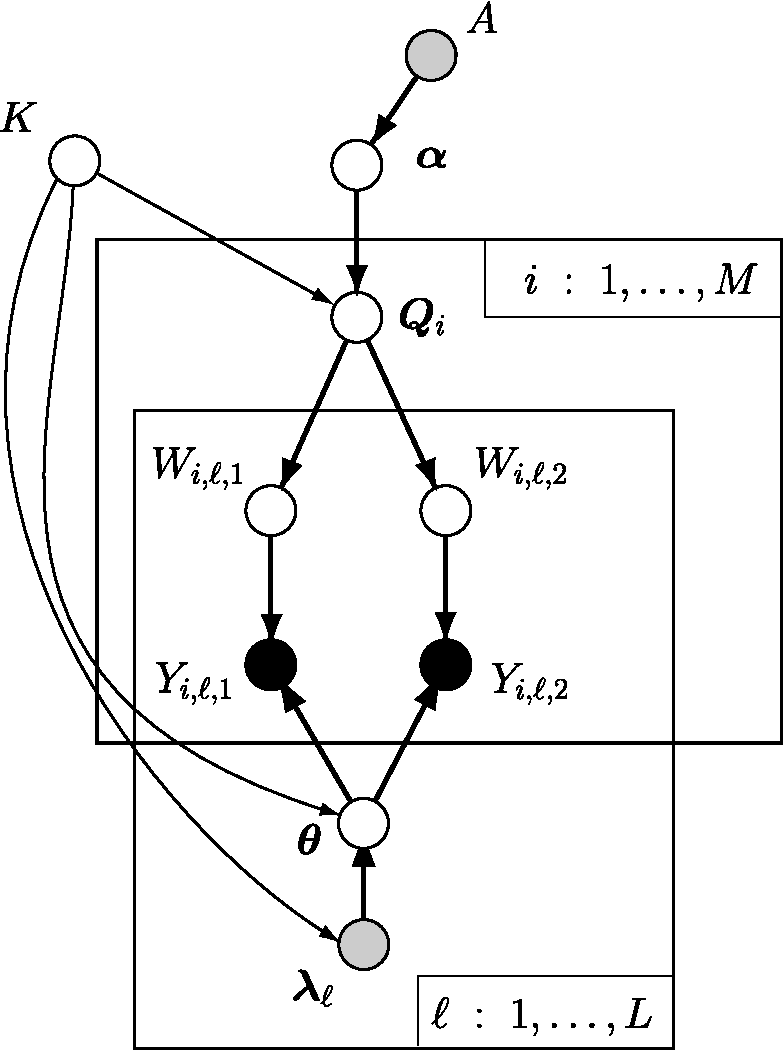
\includegraphics[width=.61\textwidth]{illus/PritchSimpleWithK.pdf}
\end{center}
\end{minipage}



\newslide{Traversing state spaces of differing dimensions---reversible jump MCMC}
\begin{itemize}
\item This is non-trivial because it involves jumping between spaces of different dimensions.
\item Requires the ``reversible jump" algorithm of Green (1995).
\end{itemize}
\begin{center}
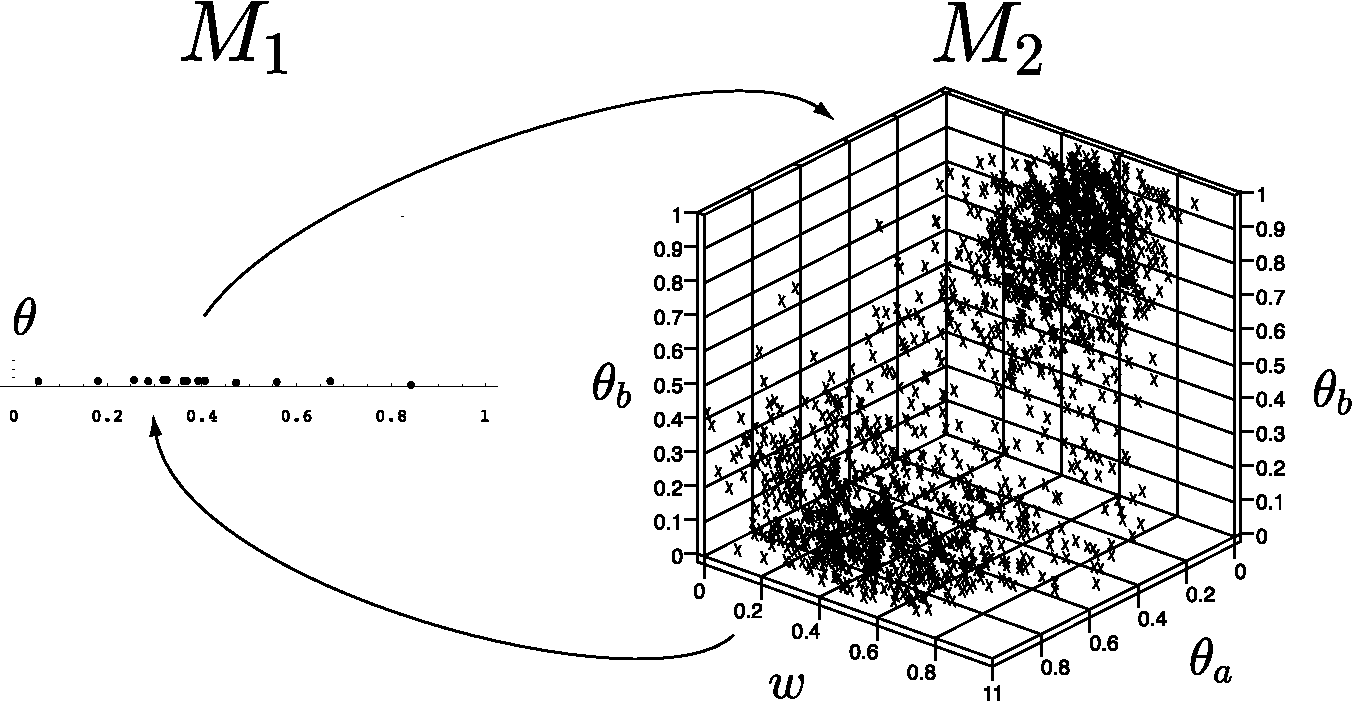
\includegraphics[width=.8\textwidth]{illus/jumpbetween.pdf}
\end{center}

%\newslide{Brief sketch of RJMCMC method}
%\begin{center}
%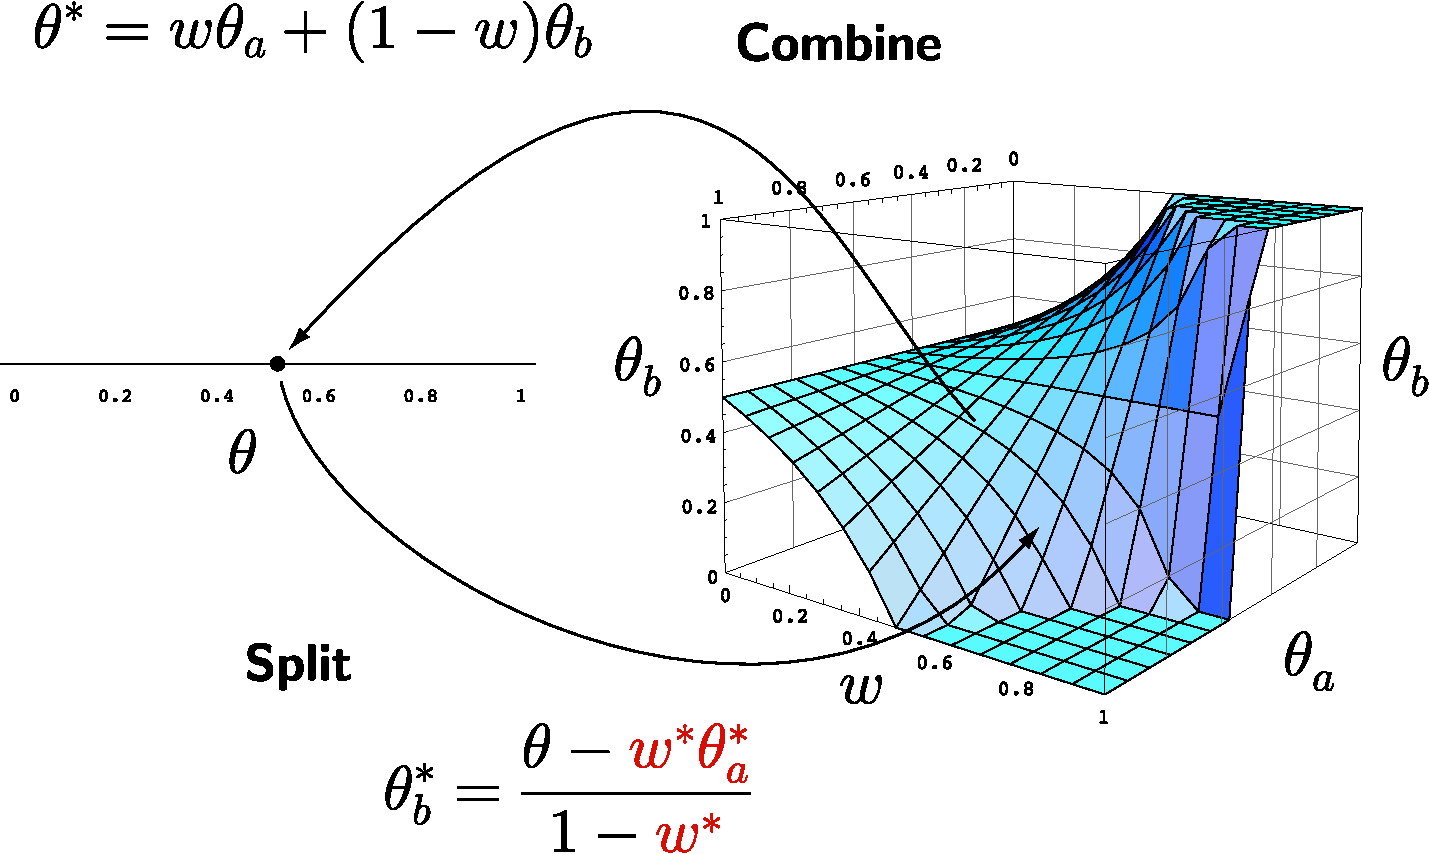
\includegraphics[width=.92\textwidth]{illus/det_trans_surface.pdf}
%\end{center}

\newpage
Unfortunately, in a model like that of {\em structure}, with numerous multiallelic loci, going from $K=2$ to $K=3$ increases the dimensionality dramatically, and RJMCMC is very difficult to apply successfully in such a situation.  

The problem is that it is very hard to propose reasonable values of the allele frequencies for the ``new" subpopulations that get added when $K$ is increased.

\newslide{How {\em structure} tries to solve the problem of choosing $K$}

Instead of computing the BF, {\sl structure} introduced a different approach to model choice.

The approach is motivated by an attempt to ``estimate" the normalizing constants
that appear in the BF. As such the output of structure includes quantities that are
labelled as estimates of $\log \Pr(Y | K)$.

However, the authors note that these estimates are unlikely to be accurate. 

Selecting
$K$ by choosing $K$ that maximises these estimates should be viewed as an {\it ad hoc}
and computationally convenient approach to model choice, that performed well 
in simulations.

\newslide{How {\em structure} tries to solve the problem of choosing $K$}

For notational convenience let's denote by $\Omega$ the latent variables $\bm{W}$, $\bm{Q}$, $\bm{\alpha}$ and $\bm{\theta}$, and denote all the observed data by $Y$.

\begin{enumerate}
\item First notice that from the law of conditional probability:
\[
	P(\Omega,Y|K) = P(Y|K,\Omega)P(\Omega|K)
\]
it follows that:
\[
	P(\Omega|K) = \frac{P(\Omega,Y|K)}{P(Y|K,\Omega)}
\]
\item Then because probability distributions integrate to one:
\[
	1 = \int_\Omega P(\Omega|K)d\Omega = \int_\Omega \frac{P(\Omega,Y|K)}{P(Y|K,\Omega)} d\Omega
\]
\newpage
\item Then, write the numerator of the right side above as a product of densities, and rearrange:
\[
	1 = \int_\Omega \frac{P(\Omega|Y,K)P(Y|K)}{P(Y|K,\Omega)} d\Omega 
\]
implies
\[
	\frac{1}{P(Y|K)} = \int_\Omega \frac{P(\Omega|Y,K)}{P(Y|K,\Omega)} d\Omega =
	\int_\Omega \left(\frac{1}{P(Y|K,\Omega)}\right) P(\Omega|Y,K)
\]
\item The above can be recognized as an expectation
\[
	\int_\Omega \left(\frac{1}{P(Y|K,\Omega)}\right) P(\Omega|Y,K) = \Exp\left[\left.
	\frac{1}{P(Y|K,\Omega)}\right| Y,K\right]
\]
\item And so approximated by Monte Carlo:
\[
\approx \frac{1}{n}\sum_{i=1}^n \frac{1}{P(Y|K,\Omega^{(i)})}
\]
where $\Omega^{(i)}$ is simulated from its conditional distribution given $Y$ and $K$.  This is precisely the sort of sample that doing MCMC in {\em structure} at a fixed value of $K$ gives you.   
\item Unfortunately, this Monte Carlo estimator, known as the ``harmonic mean" estimator, is notoriously unstable and may have infinite variance.
\item Instead, consider the random variable $D = -2\log P(Y|\Omega,K)$ (the ``deviance") which is a function of the random variable $\Omega$.  Assume that $D$ (conditional on the data) is normally distributed (an ``admittedly dubious" assumption).
\item Going back to our harmonic mean expectation, we can write it in terms of D:
\[
	\frac{1}{P(Y|K)} = \Exp\left[\left.
	\frac{1}{P(Y|K,\Omega)}\right| Y,K\right] = 
	\Exp[e^{D/2}]
\]
\item If $D$ really is normally distributed then the right hand side of the above equation is just the moment generating function for a normal random variable (recall that $\Exp[e^{tX}] = e^{\mu t + \sigma^2 t^2/2}$).
\item So:
\[
	\frac{1}{P(Y|K)} = e^{\mu/2 + \sigma^2/8} \Rightarrow -\log P(Y|K) = \mu/2 + \sigma^2/8
\] 
where $\mu=\Exp[D|Y]$ and $\sigma^2 = \Var[D|Y]$.
\item Finally, it is easy to estimate $\mu$ and $\sigma$ by Monte Carlo from the values of $D^{(i)}$ obtained when the chain samples from the values of $\Omega^{(i)}$. 
\end{enumerate}


\newslide{Deviance Information Criterion (DIC)}

%In $C_p $ , AIC and BIC it is assumed that the ``number of
%parameters" is a well-defined concept. It is taken to be
%synonymous with the model degrees of freedom or the number of free
%parameters.

%In a Bayesian analysis the prior effectively acts to restrict the
%freedom of these parameters to some extent and thus the
%appropriate model degrees of freedom is less clear.
%\es\bs

Spiegelhalter et. al. (2002) have proposed an alternative method
for selecting models based on MCMC output, called the ``Deviance
Information Criterion" (DIC).

In common with the {\sl structure} approach, DIC also
involves penalising the mean deviance, but with a different penalty.

Unpublished simulations from Carlos Bustamante suggest that DIC may
perform better at selecting $K$ than the current approach implemented
in {\sl structure}, and this approach may be implemented in future versions.

%    \[
%p_D  = \overline {D(\theta )}  - D\left( {\bar \theta } \right)
%\]

%
%where $D(\theta ) =  - 2\log\left( {p(y|\theta )} \right) +
%2\log\left( {K(y)} \right)$
% is the deviance and $K(y)$
% is a function that does not depend on $\theta $
%, i.e.

%\begin{eqnarray*}
%\mbox{Effective degrees of freedom } &=& \mbox{Posterior Mean
%Deviance}\\
%&&-\mbox{Deviance at posterior mean}
%\end{eqnarray*}
%\es\bs

%They also suggest that the posterior mean
%deviance,$\overline{D(\theta )}$, can be used as a measure of
%model adequacy.

%Finally they ``tentatively" suggest adding $p_D$
% and $\overline{D(\theta )}$
% to give a Deviance Information Criterion which may be used
%for model comparison:

%\[
%{\rm DIC} = D(\theta ) + p_D
%\]

%
%In the case of linear models with vague priors DIC
%corresponds to AIC.
%\es\bs

%
%In models with hyper-parameters (e.g. hierarchical models) it
%makes a difference whether you regard the hyper-parameters
%as part of the model specification (i.e. the likelihood) or part of
%the prior.

%In some case it is possible for $p_D  < 0$!

%The jury is still out on how useful $p_D $ and DIC are for model
%comparison.


\newslide{Thermodynamic Integration}
A very recent paper in {\em Genetics}
\begin{center}
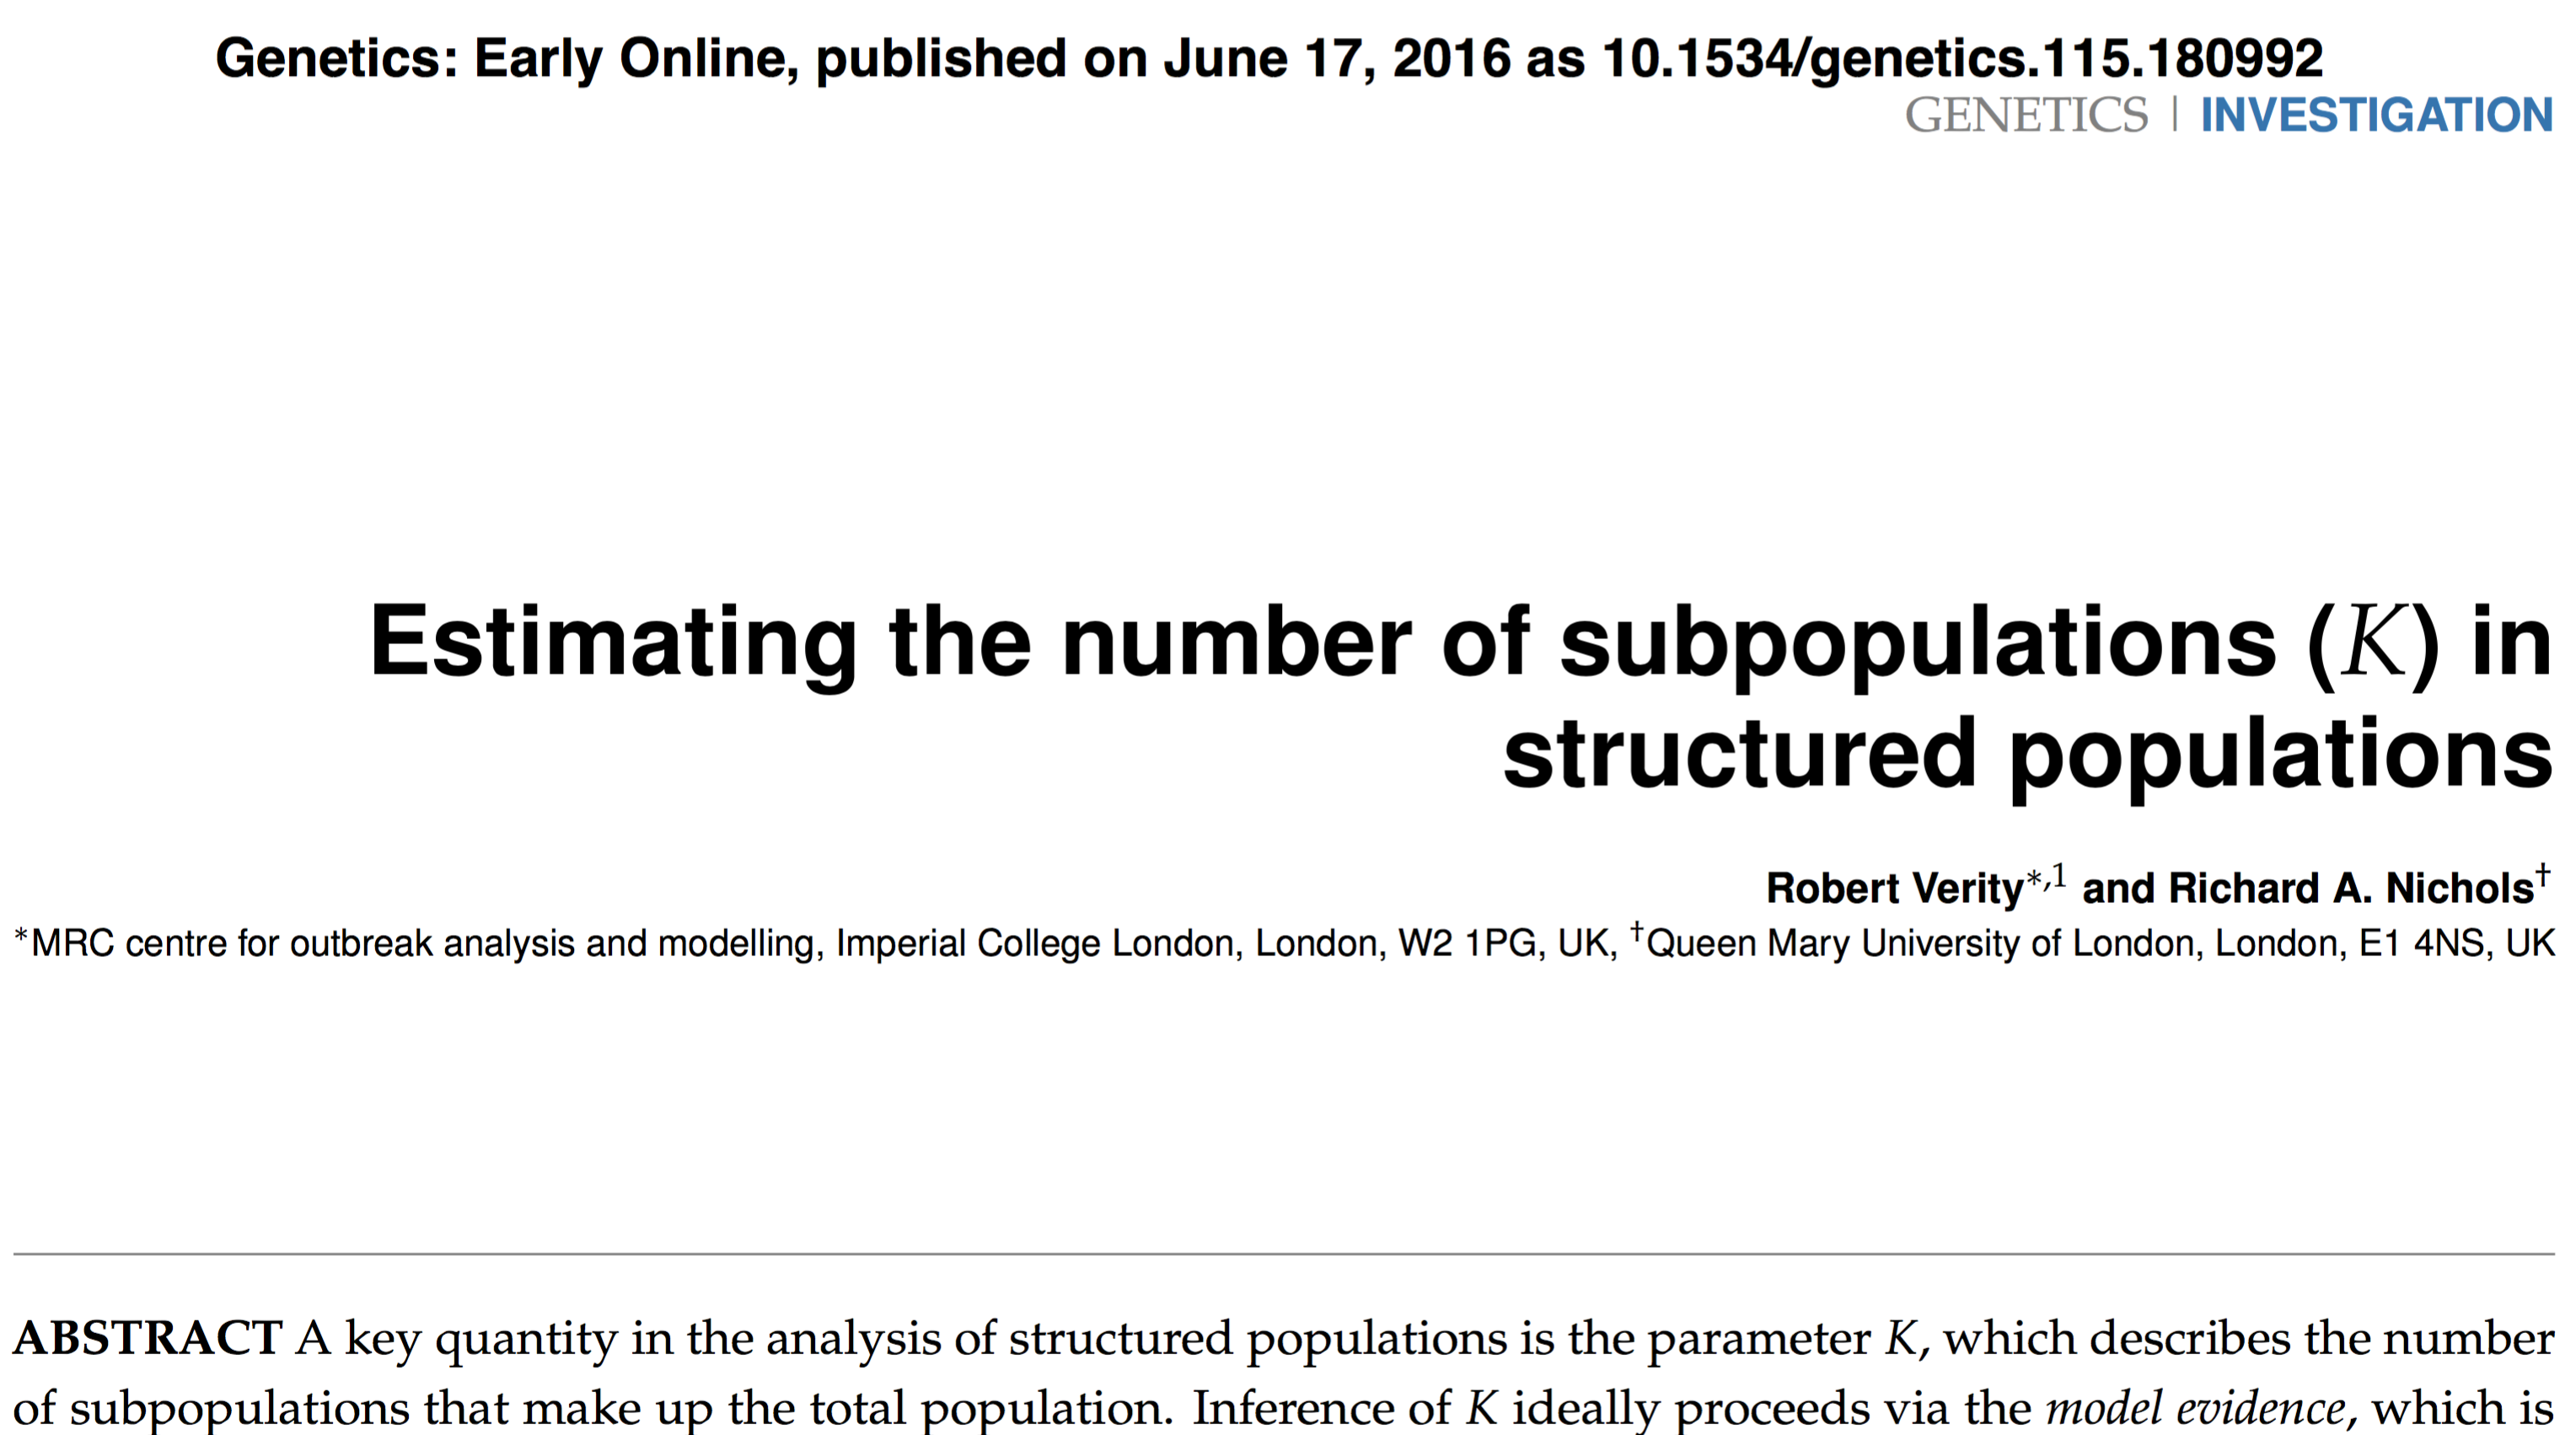
\includegraphics[width = 0.9\textwidth]{illus/verity.png}
\end{center}
\newpage

These authors show some oft-observed behavior of {\em structure}'s estimator of the $\log P(\mathrm{Data} | K)$---the values keep climbing as $K$ gets larger:
\begin{center}
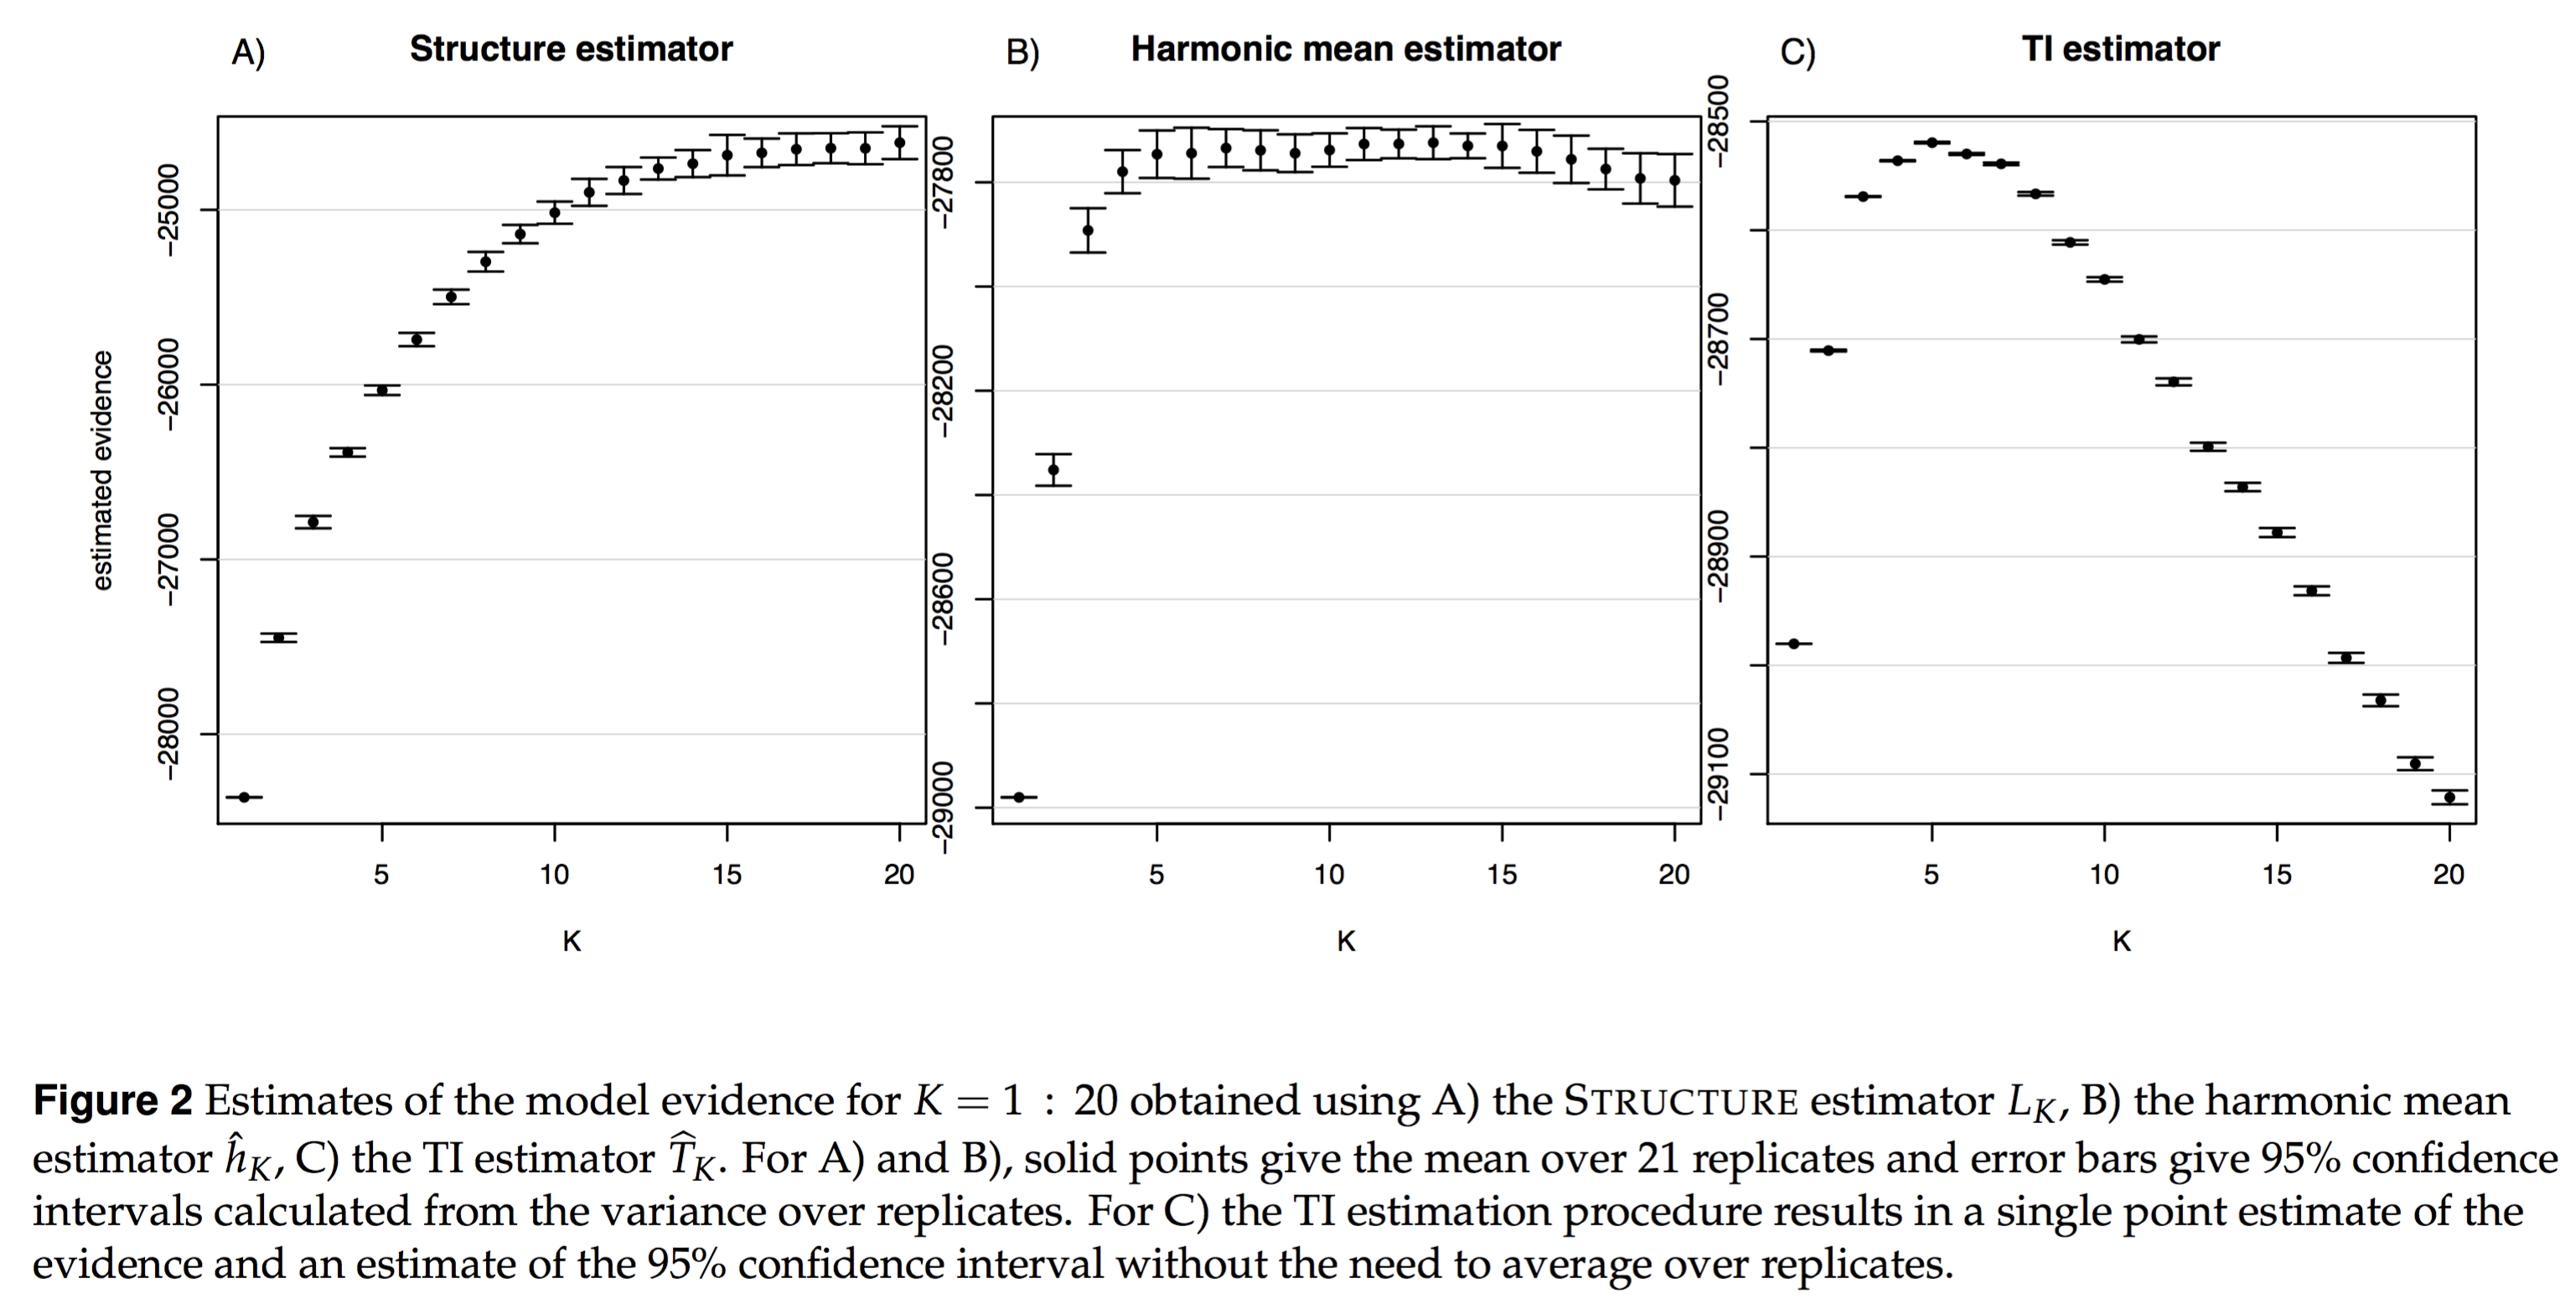
\includegraphics[width = 0.9\textwidth]{illus/verity2.png}
\end{center}
$\bullet$ And their thermodynamic integration approach seems to give a more stable, reasonable 
result (confirmed in simulations, as well).

\newpage
ECA has prepared a short(-ish) and still incomplete R-notebook describing the thermodynamic inegration method.  It is available at:

{\tiny
\url{https://github.com/eriqande/sisg_mcmc_course/blob/master/rmarkdown/thermodynamic-integration/thermodynamic-integration.nb.html}
}

\newslide{Summary}

\begin{itemize}
\item Avoid drawing strong conclusions based solely on
choice of $K$ indicated by a {\sl structure} analysis.
\item Whenever you come across a Bayes Factor, ask yourself whether the priors
used are sensible, and how they might influence the result.
\end{itemize}

\end{document}
